%\begin{frame}{LU decomposition problem}
%\begin{columns}[c]
%\begin{column}{0.02\textwidth}
%\end{column}
%\begin{column}{0.45\textwidth}
%\begin{tabbing}
%Let be $A$ a $n*n$ square matrix\\
%For \= $k$ from $1$ to $n$\\
%\>\visible<3->{\alert{Search for pivot then swap}}\\
%\> For \=$i$ from $k+1$ to $n$\\
%\>\> $a_{i,k} = a_{i,k}/a_{k,k}$\\
%\> For \=$i$ from $k+1$ to $n$\\
%\>\> For \=$j$ from $k+1$ to $n$\\
%\>\>\> $a_{i,j} = a_{i,j}-a_{i,k}*_{k,j}$\\
%\end{tabbing}
%\end{column}
%\begin{column}{0.02\textwidth}
%\end{column}
%\begin{column}{0.45\textwidth}
%\begin{itemize}
%\item $a_{k,k}$ may be close to zero
%\item Numerical value may be deteriorated due to fixed precision used by computers
%\end{itemize}
%\pause
%$\Rightarrow$ LU decomposition is not stable
%\end{column}
%\end{columns}
%\visible<3>{\alert{Solution is pivoting}}
%\end{frame}
%
%\begin{frame}{Partial Pivoting Algorithm}
%
%{
%The partial pivoting consist to look for the element with the maximal absolute value on the $k^{th}$ column from $a_{k,k}$, then swap its row with the row consisting $a_{k,k}$.
%}
%{
%The partial pivoting is:
%\begin{itemize}
%\item Practically stable and accurate
%\item Commonly used in the scientific community
%\item Used in the LINPACK benchmark to rank the TOP 500 super-computers
%\end{itemize}
%}
%\pause
%\begin{exampleblock}{Problem:}
%Complex to adapt to the task flow model
%\end{exampleblock}{}
%\end{frame}

\subsection{Panel Factorization}

\begin{frame}{Panel Factorization Problems}
\framesubtitle{Tasks of panel factorization}
\begin{center}
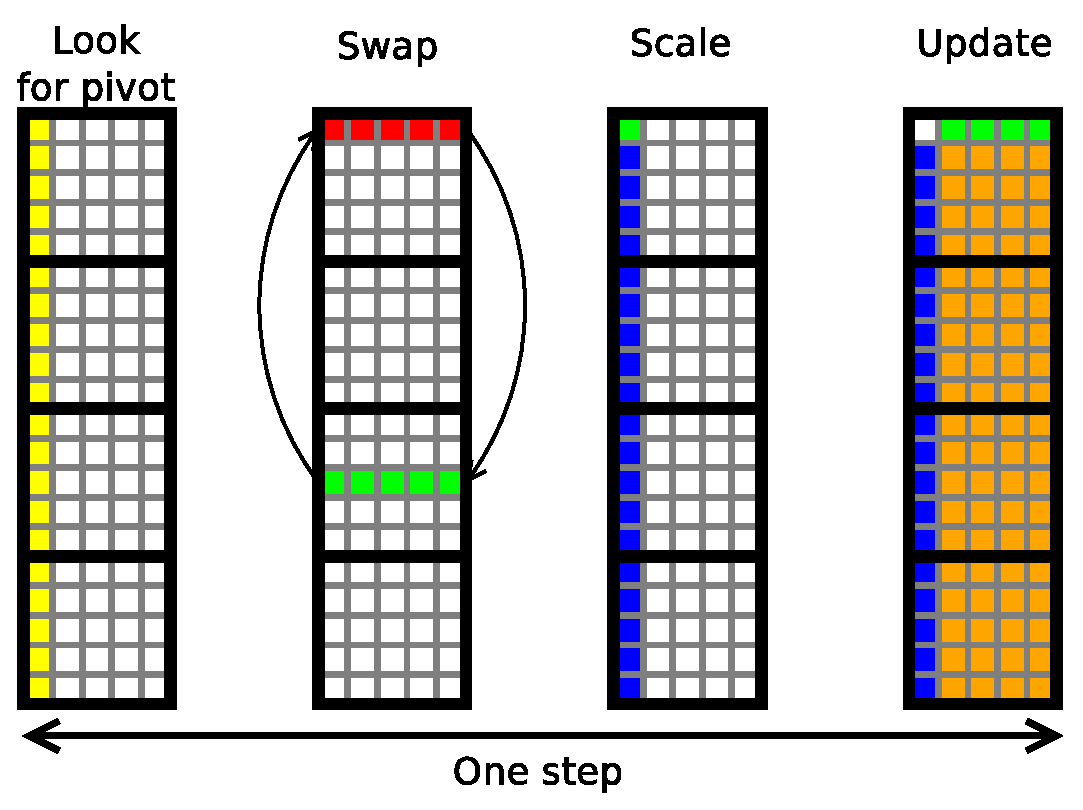
\includegraphics[width=0.6\textwidth]{panel_operation}
\end{center}
\begin{center}
\pause
\begin{itemize}
\item \alert{Look for a pivot is distributed over several tiles}
\item \alert{Tasks are fine grained}
\end{itemize}
\end{center}
\end{frame}

\begin{frame}{Panel Factorization Problems}
\framesubtitle{Reduce fine grained tasks}
\begin{center}
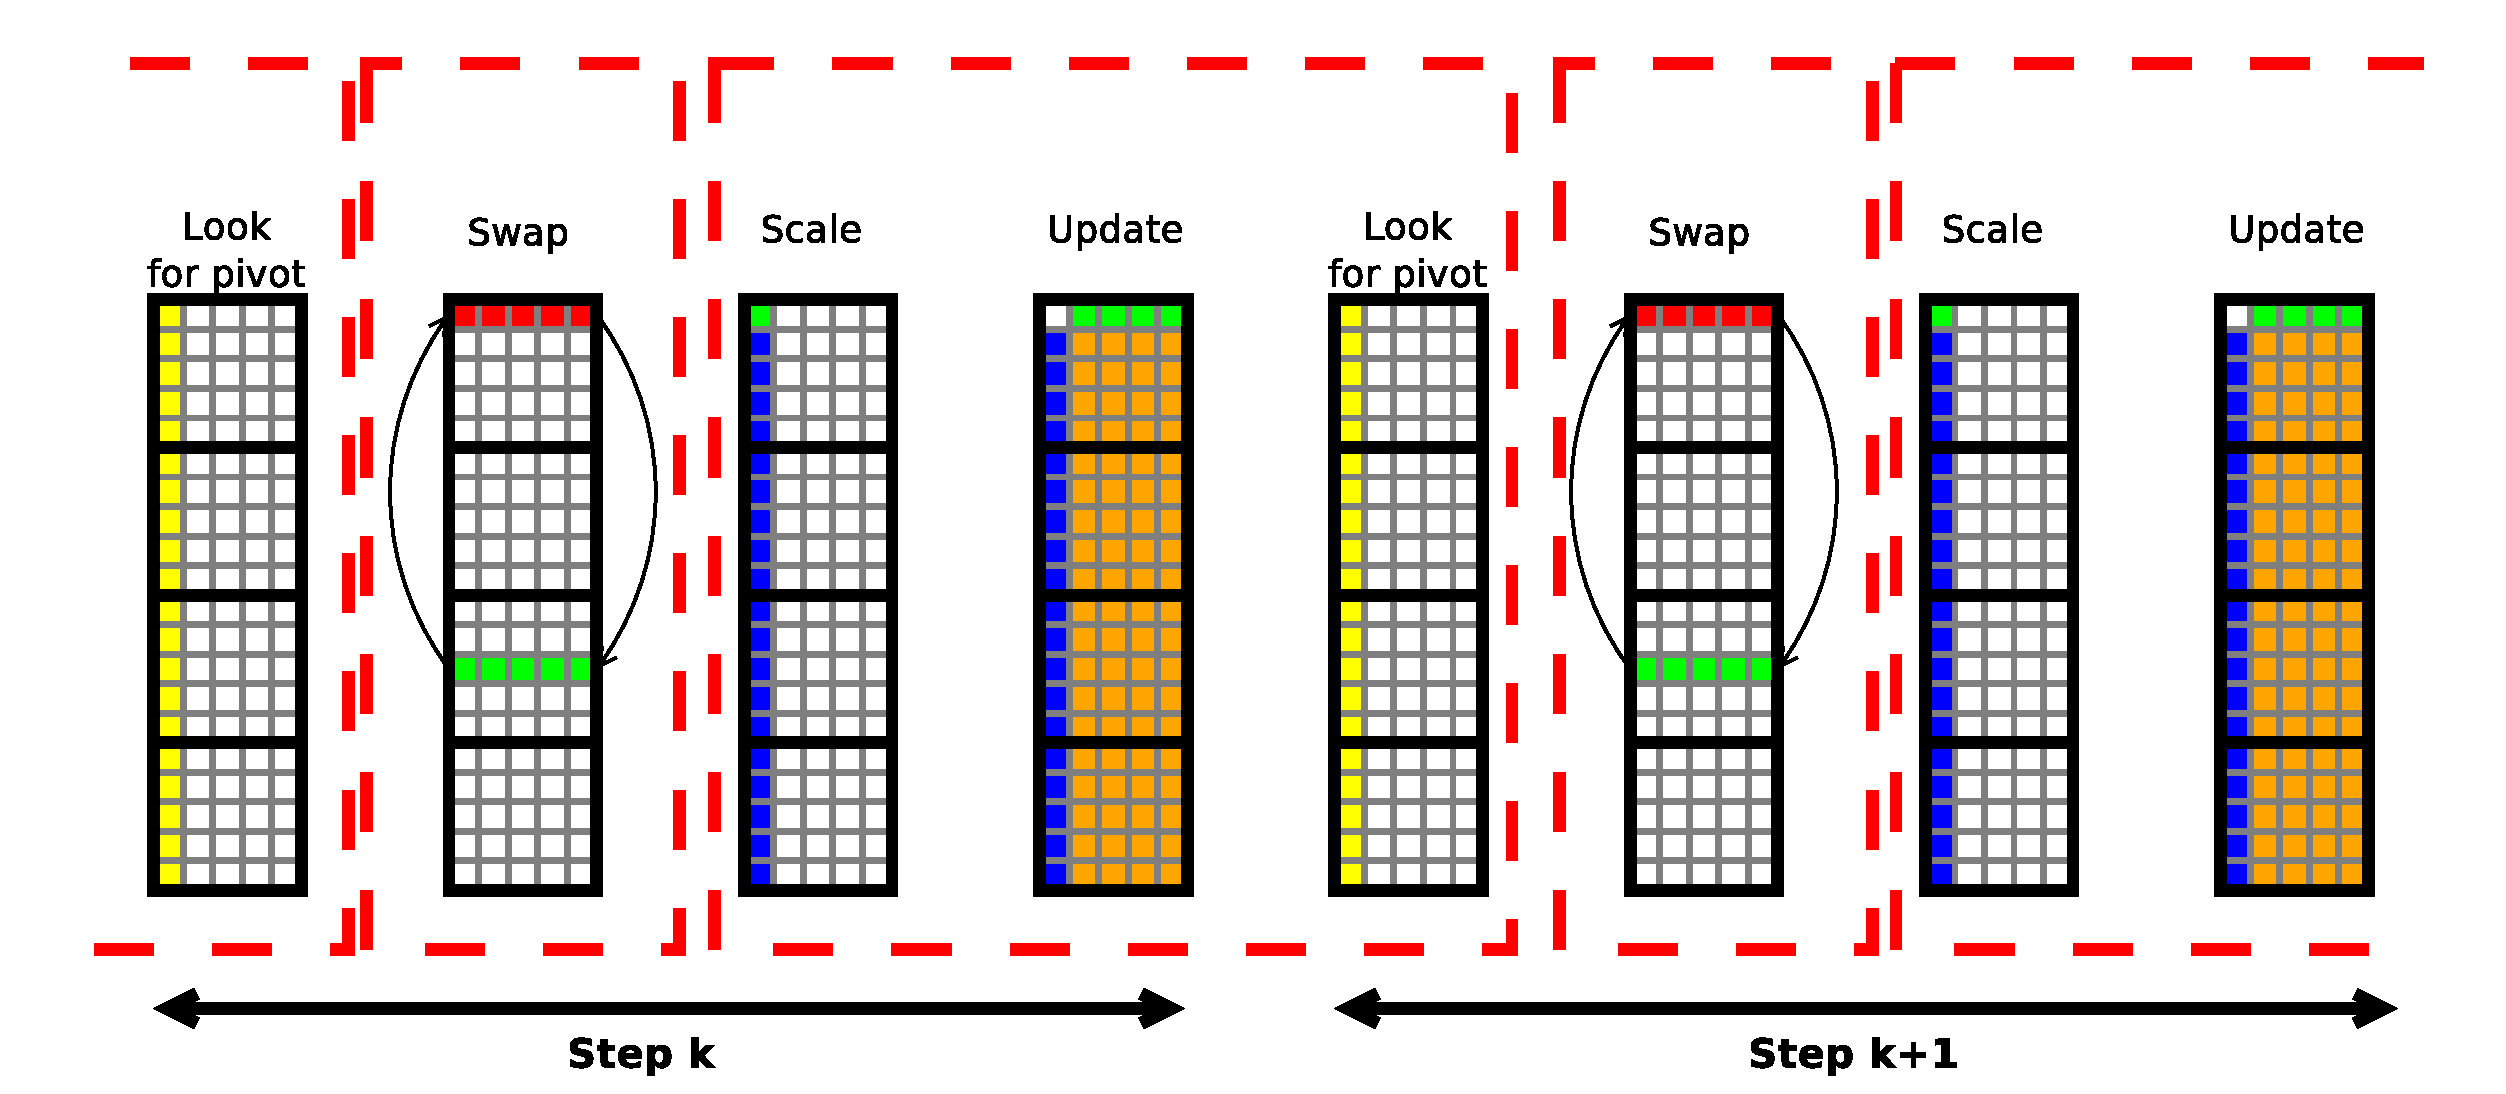
\includegraphics[width=0.8\textwidth]{merge}
\end{center}
\end{frame}


\begin{frame}{Panel Factorization Problems}
\framesubtitle{Natural task flow of panel factorization}
\begin{center}
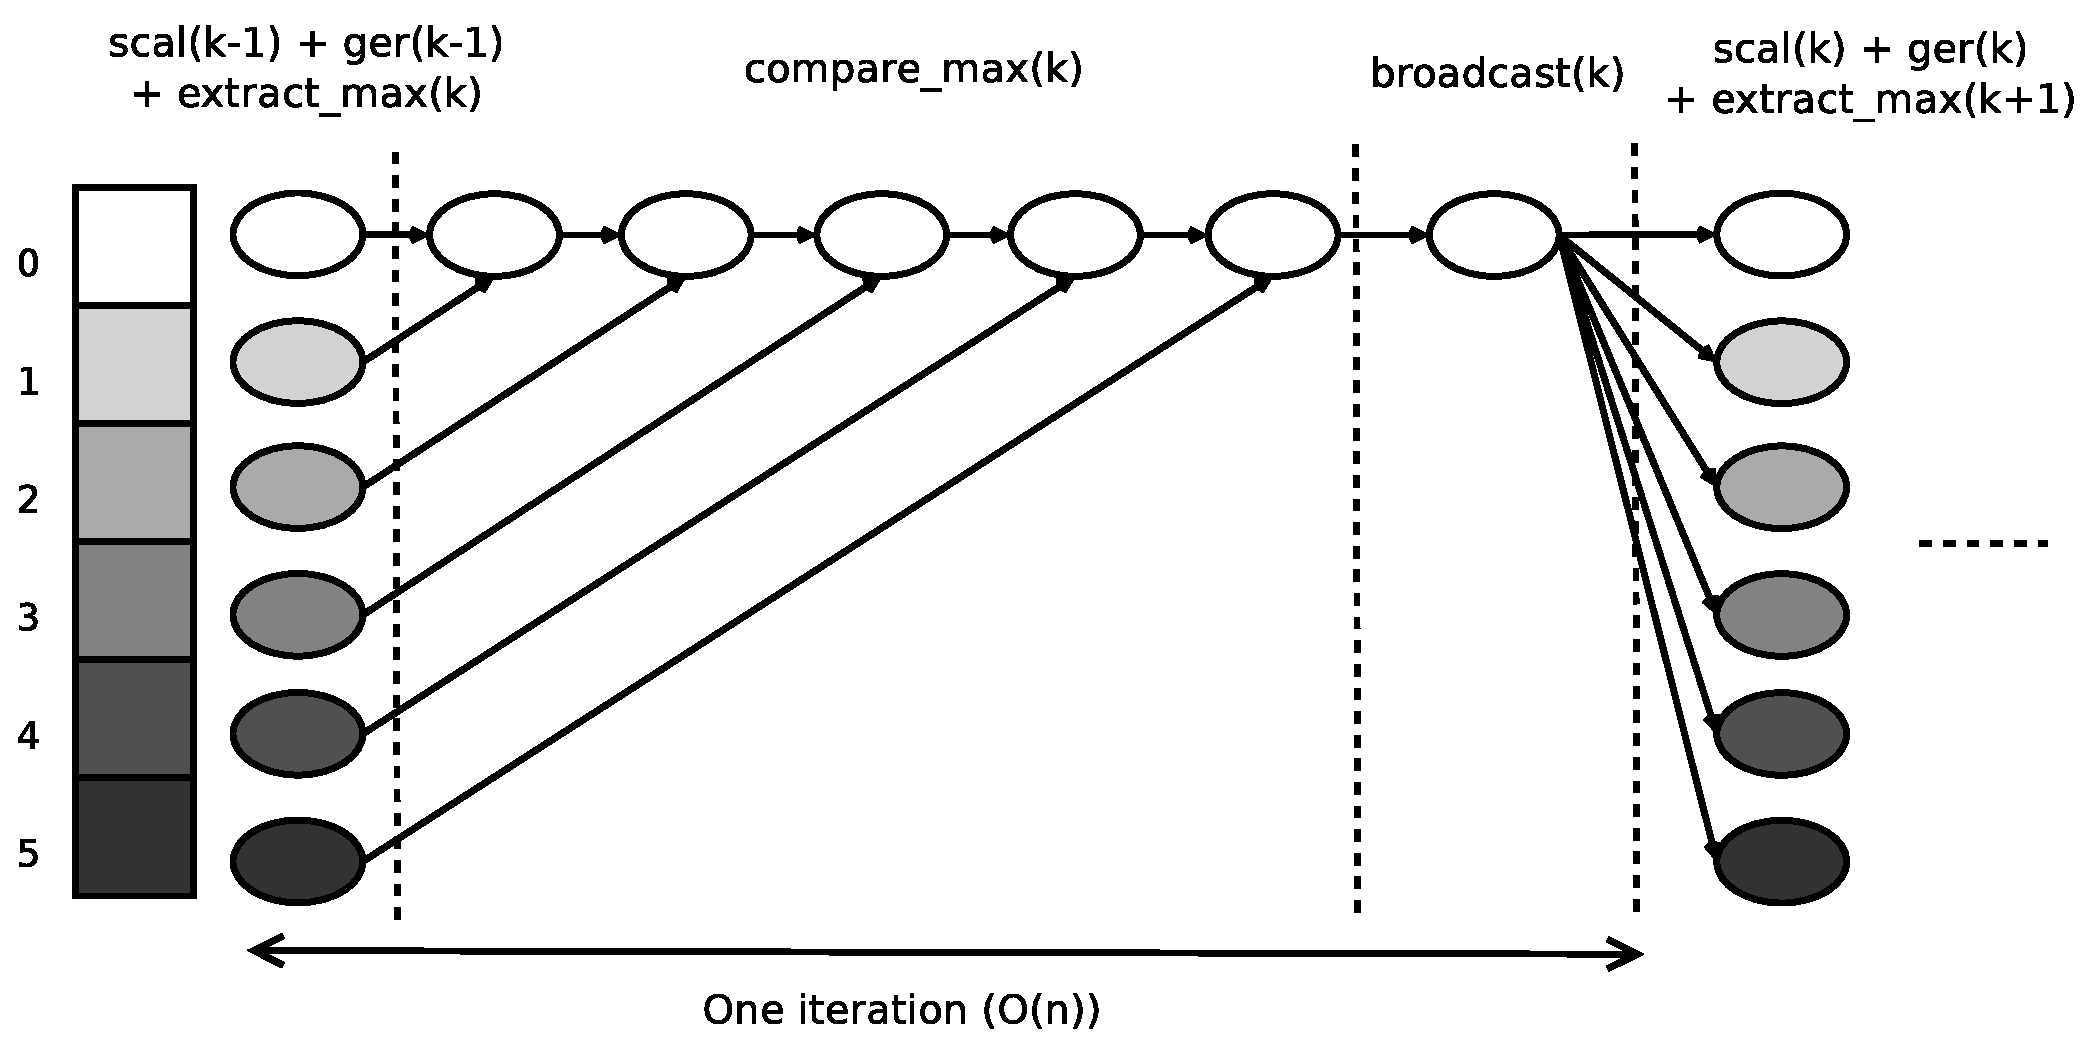
\includegraphics[width=0.6\textwidth]{natural_tf_bw}
\end{center}
\pause
\begin{center}
$\Rightarrow$ Serialized task flow!
\end{center}
\pause
\begin{exampleblock}{Optimizations:}
Use \emph{all\_reduce} operation (using Bruck's algorithm)
\end{exampleblock}{}
\end{frame}

\begin{frame}{Panel Factorization Problems}
\framesubtitle{Optimized task flow of panel factorization for distributed architectures}
\begin{center}
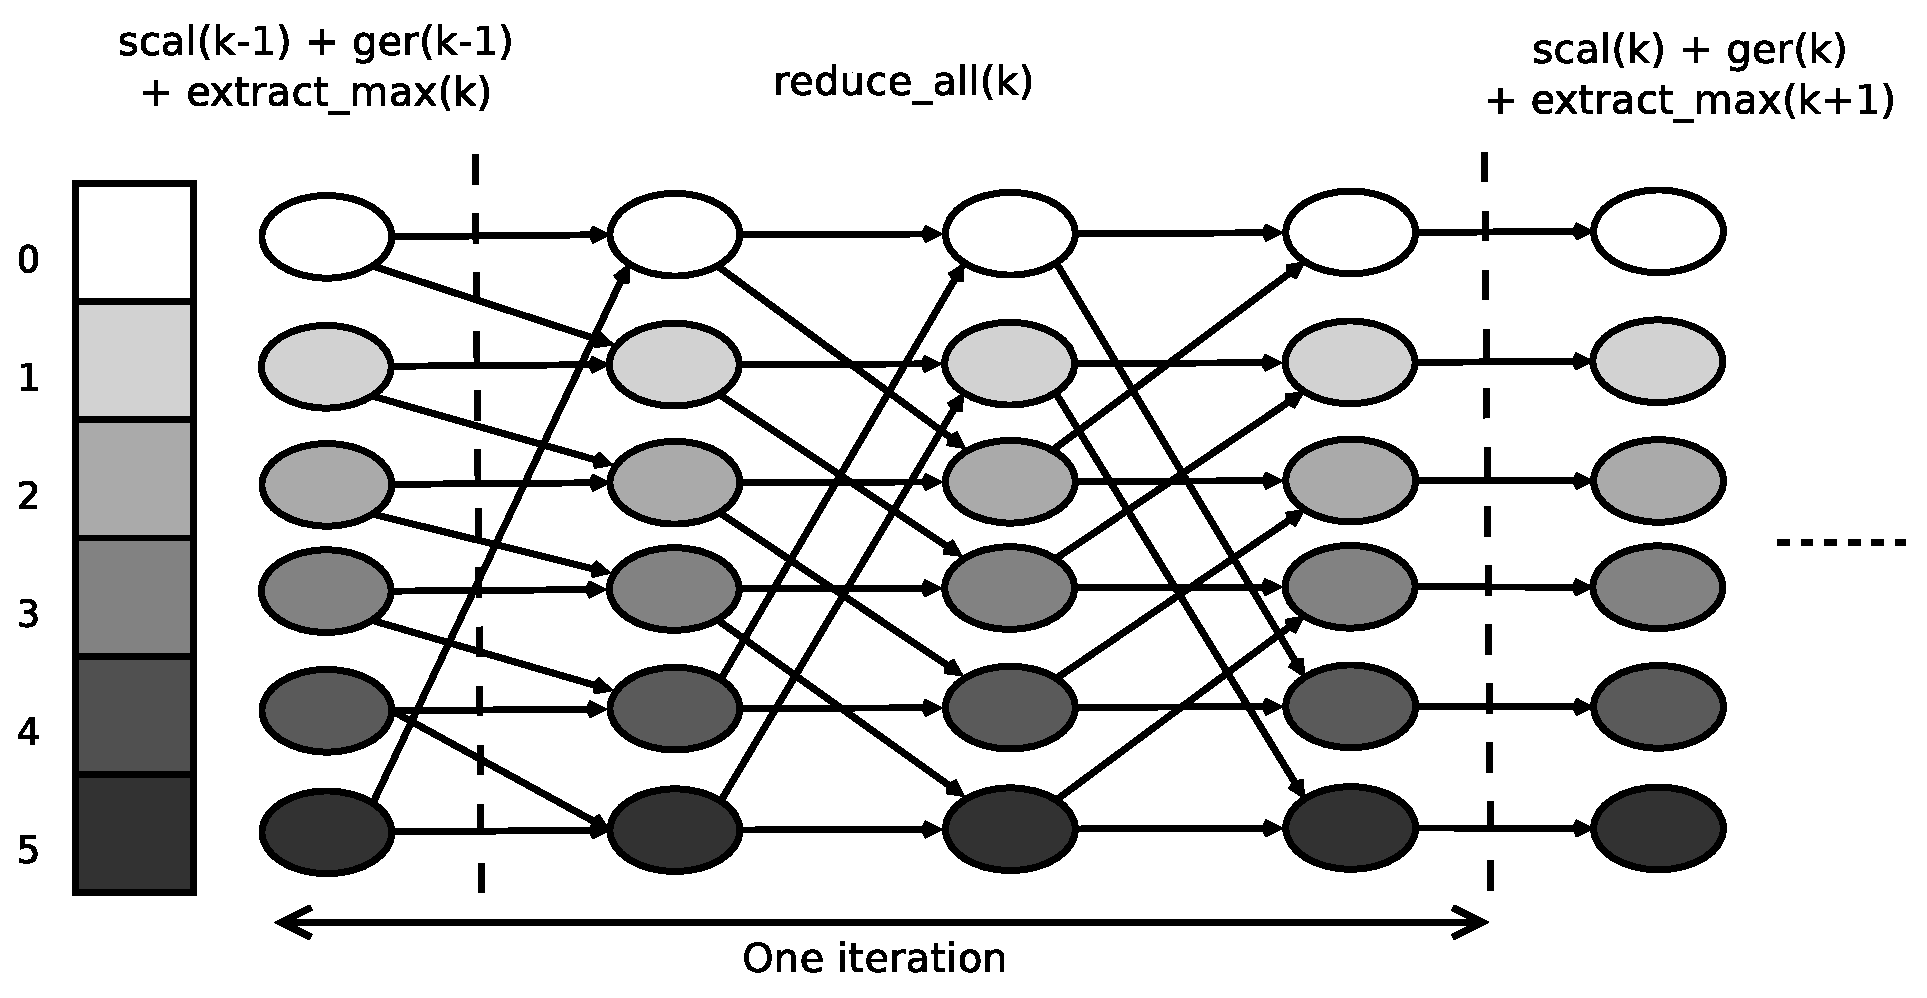
\includegraphics[width=0.6\textwidth]{distributed_tf_bw}
\end{center}
\end{frame}

\begin{frame}{Panel Factorization Problems}
\framesubtitle{Optimized task flow of panel factorization for hierarchical architectures}
\begin{center}
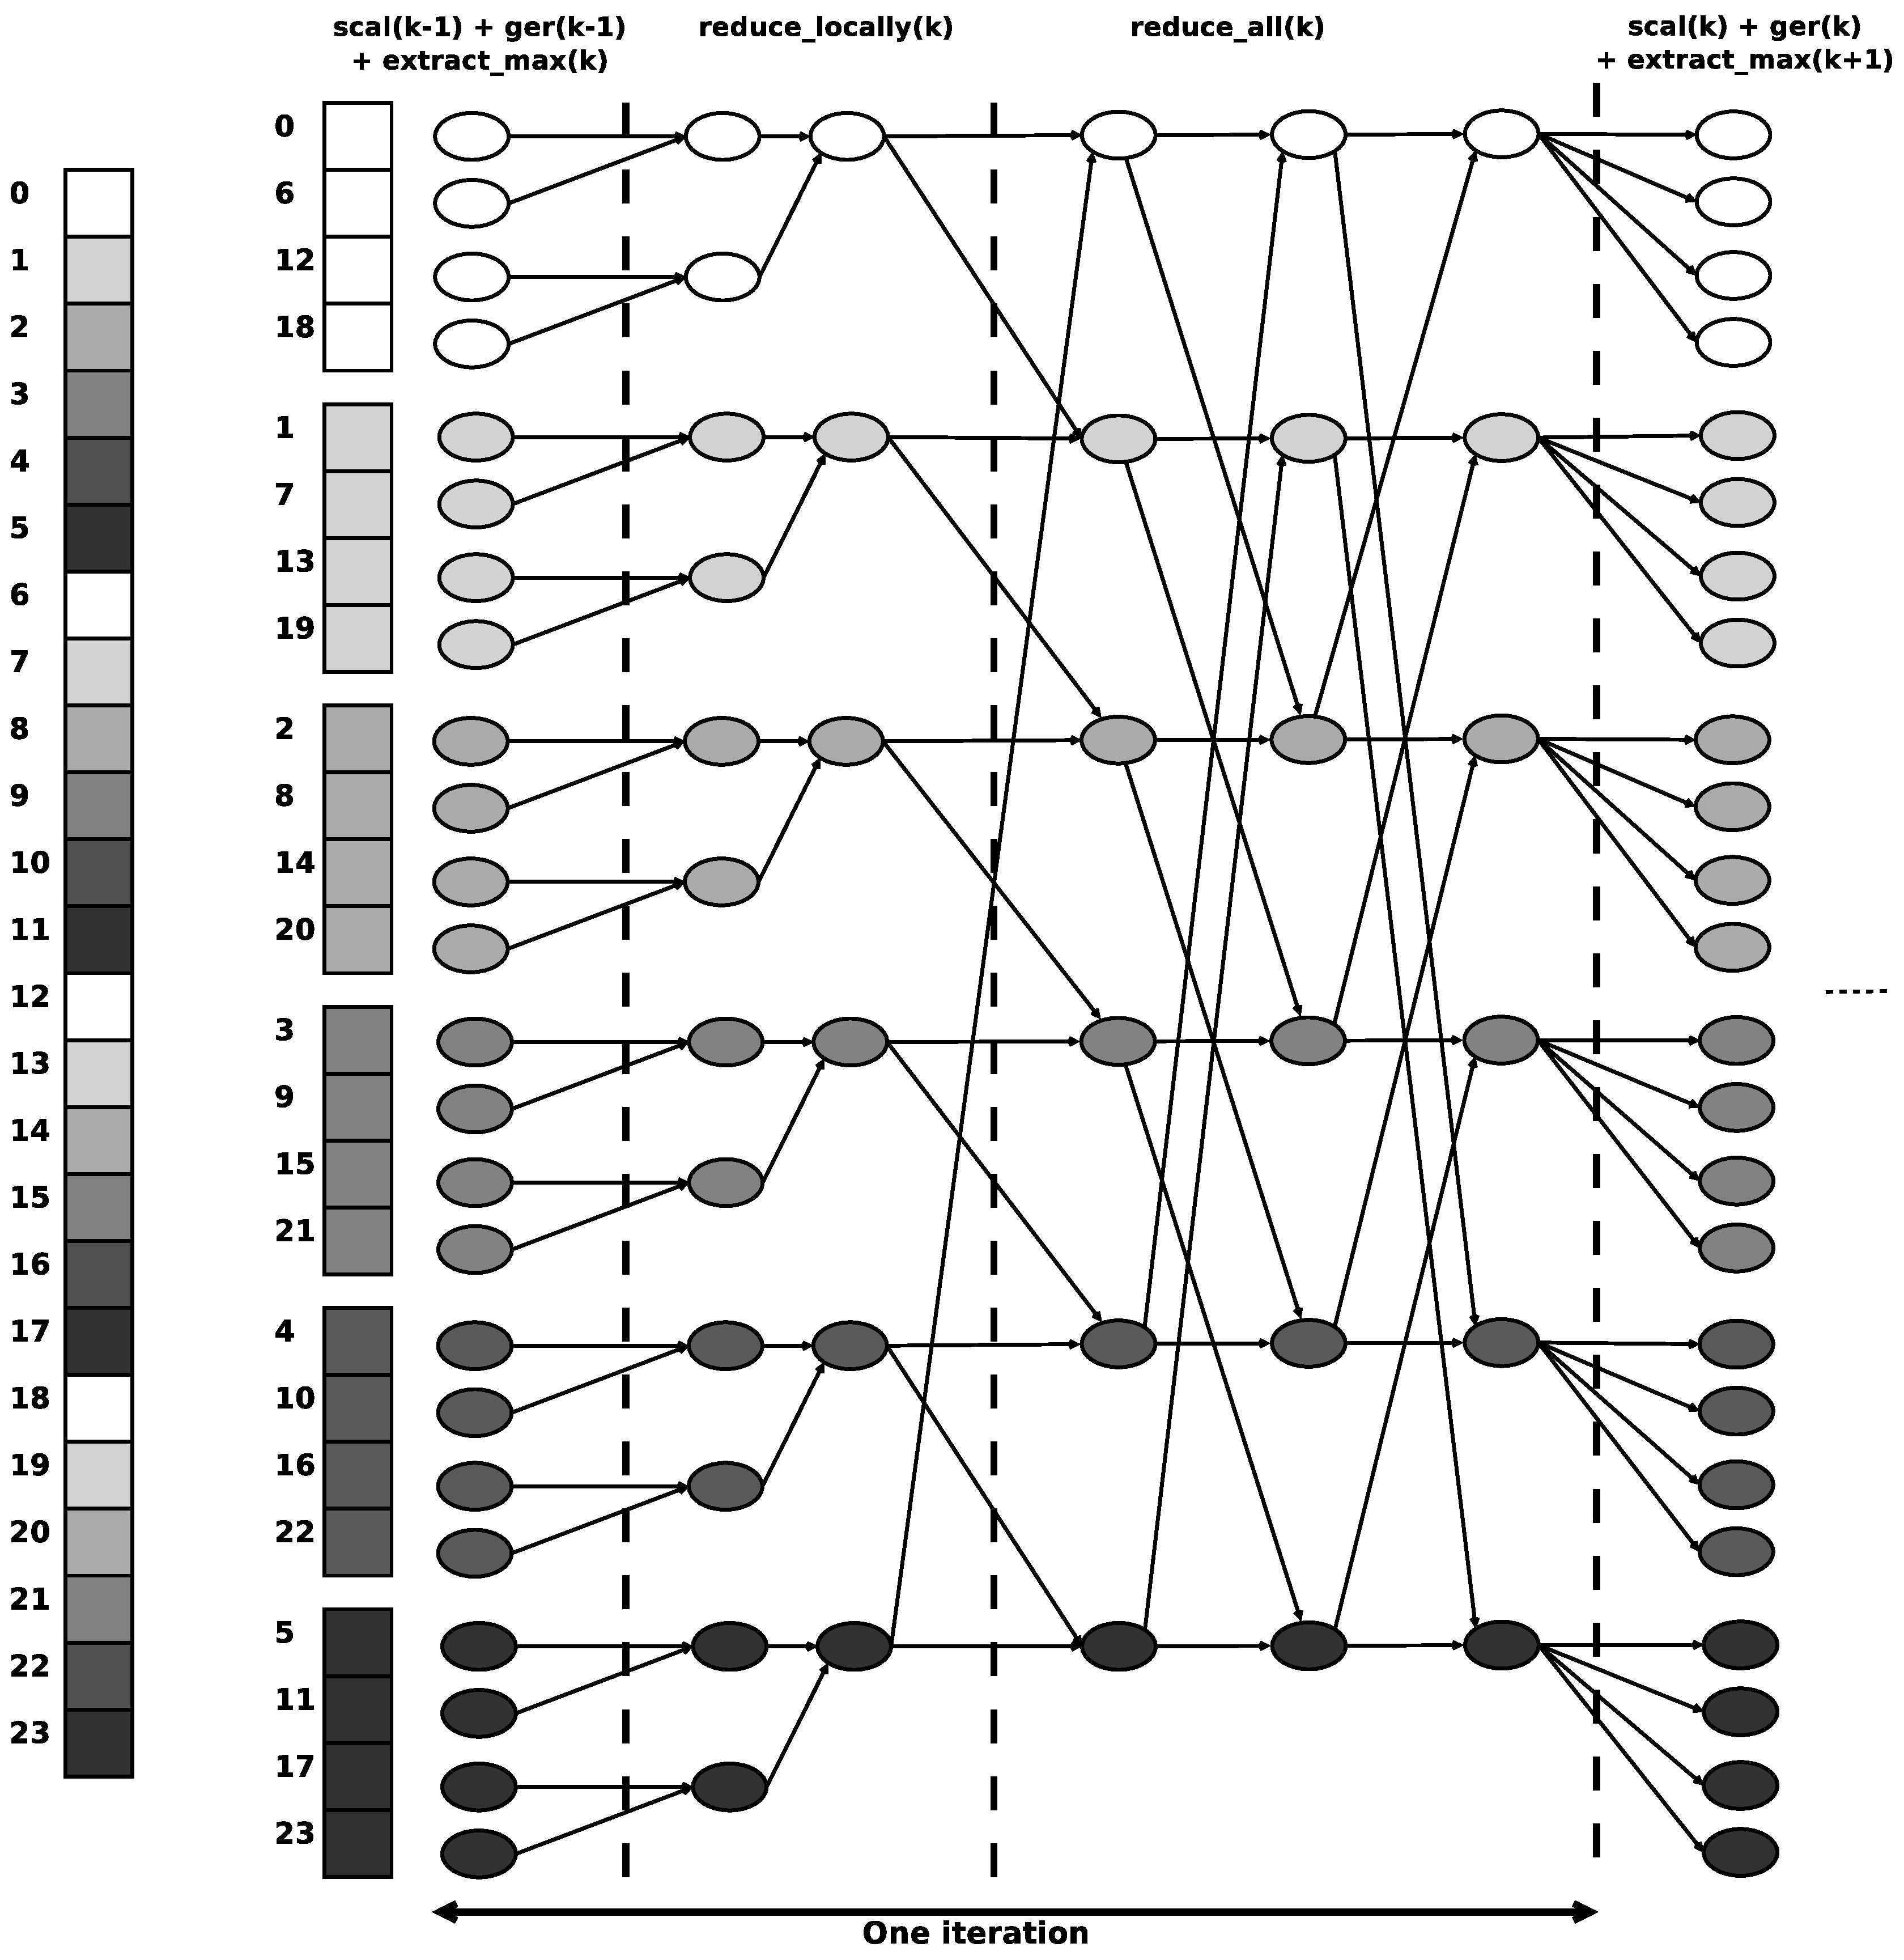
\includegraphics[width=0.55\textwidth]{hybrid_tf_bw}
\end{center}
\end{frame}

\subsection{Update of Trailing Sub-matrix}

\begin{frame}{Update Problems}
\framesubtitle{Update trailing sub-matrix}
\begin{columns}
\begin{column}{.50\textwidth}
\begin{center}
\includegraphics[scale=0.2]{update_swap.pdf}
\end{center}
\end{column}
\hfill
\begin{column}{.50\textwidth}
The upper tile exchange rows with other tile depending on pivots values.
\end{column}
\end{columns}
\pause
\begin{footnotesize}
\begin{exampleblock}{Problem}
\begin{itemize}
\item Dynamic decision for a static DAG
\pause
$\rightarrow$ Generate tasks for all possible communications?
\pause
\item Pivots implies swaps in a specific order
\pause
$\rightarrow$ Use permutation instead of pivots
\pause
\item Serialized communications
\pause
$\rightarrow$ Separate Swap from/into upper tile
\end{itemize}
\end{exampleblock}{}
\end{footnotesize}
\end{frame}

\begin{frame}{Update Problems}
\framesubtitle{Natural task flow of one swap in update}
\begin{center}
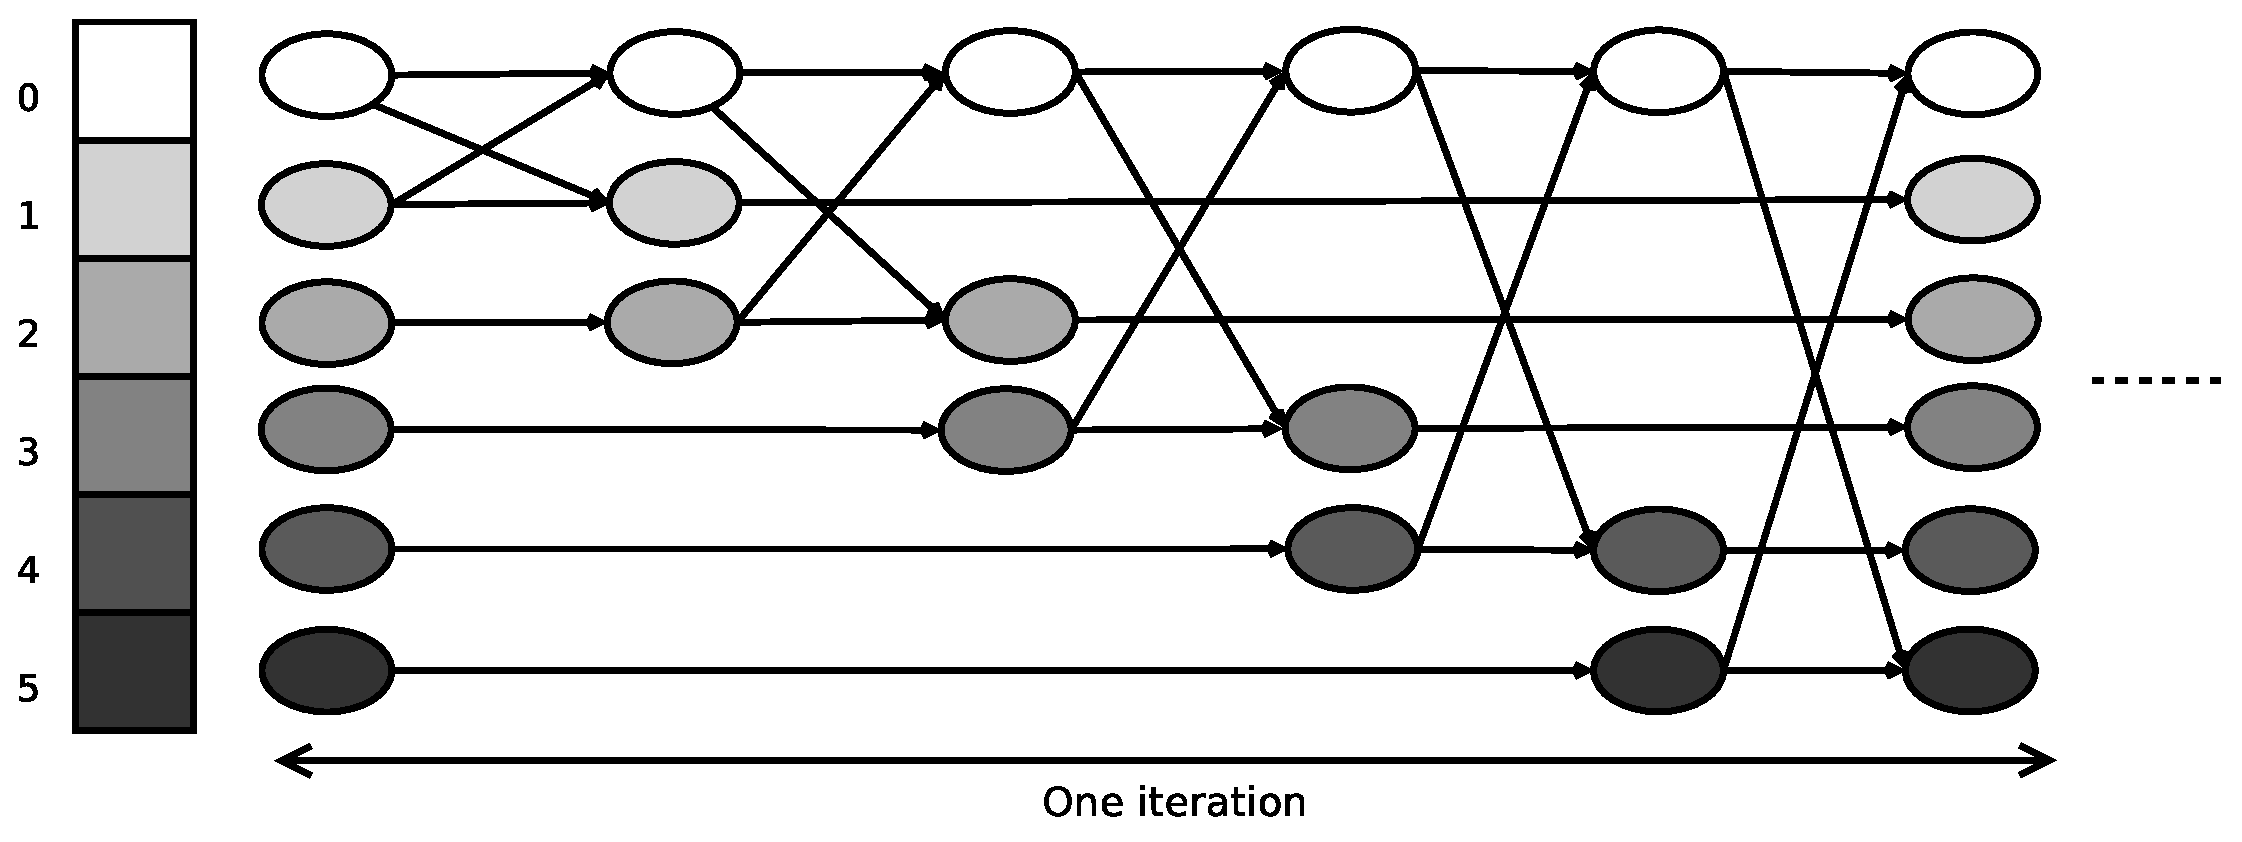
\includegraphics[width=0.6\textwidth]{natural_swap_tf_bw}
\end{center}
%\pause
%\begin{center}
%$\Rightarrow$ Huge number of synchronizations!
%\end{center}
%\pause
%\begin{exampleblock}{Optimizations:}
%Do all swaps in one single iteration by using permutations instead of pivots
%\end{exampleblock}{}
\end{frame}

\begin{frame}{Update Problems}
\framesubtitle{Optimized task flow of swaps of update for distributed architectures}
\begin{center}
\includegraphics<4>[width=0.9\textwidth]{distributed_update_tf_bw}
\end{center}

\begin{columns}
\begin{column}{.45\textwidth}
\begin{flushright}
\includegraphics<1,3>[scale=0.2]{swap_from}
\end{flushright}
\end{column}
\begin{column}{.50\textwidth}
\begin{flushleft}
\includegraphics<2,3>[scale=0.2]{swap_into}
\end{flushleft}
\end{column}
\end{columns}
\end{frame}

\begin{frame}{Update Problems}
\framesubtitle{Optimized task flow of swaps of update  for hierarchical architectures}
\begin{center}
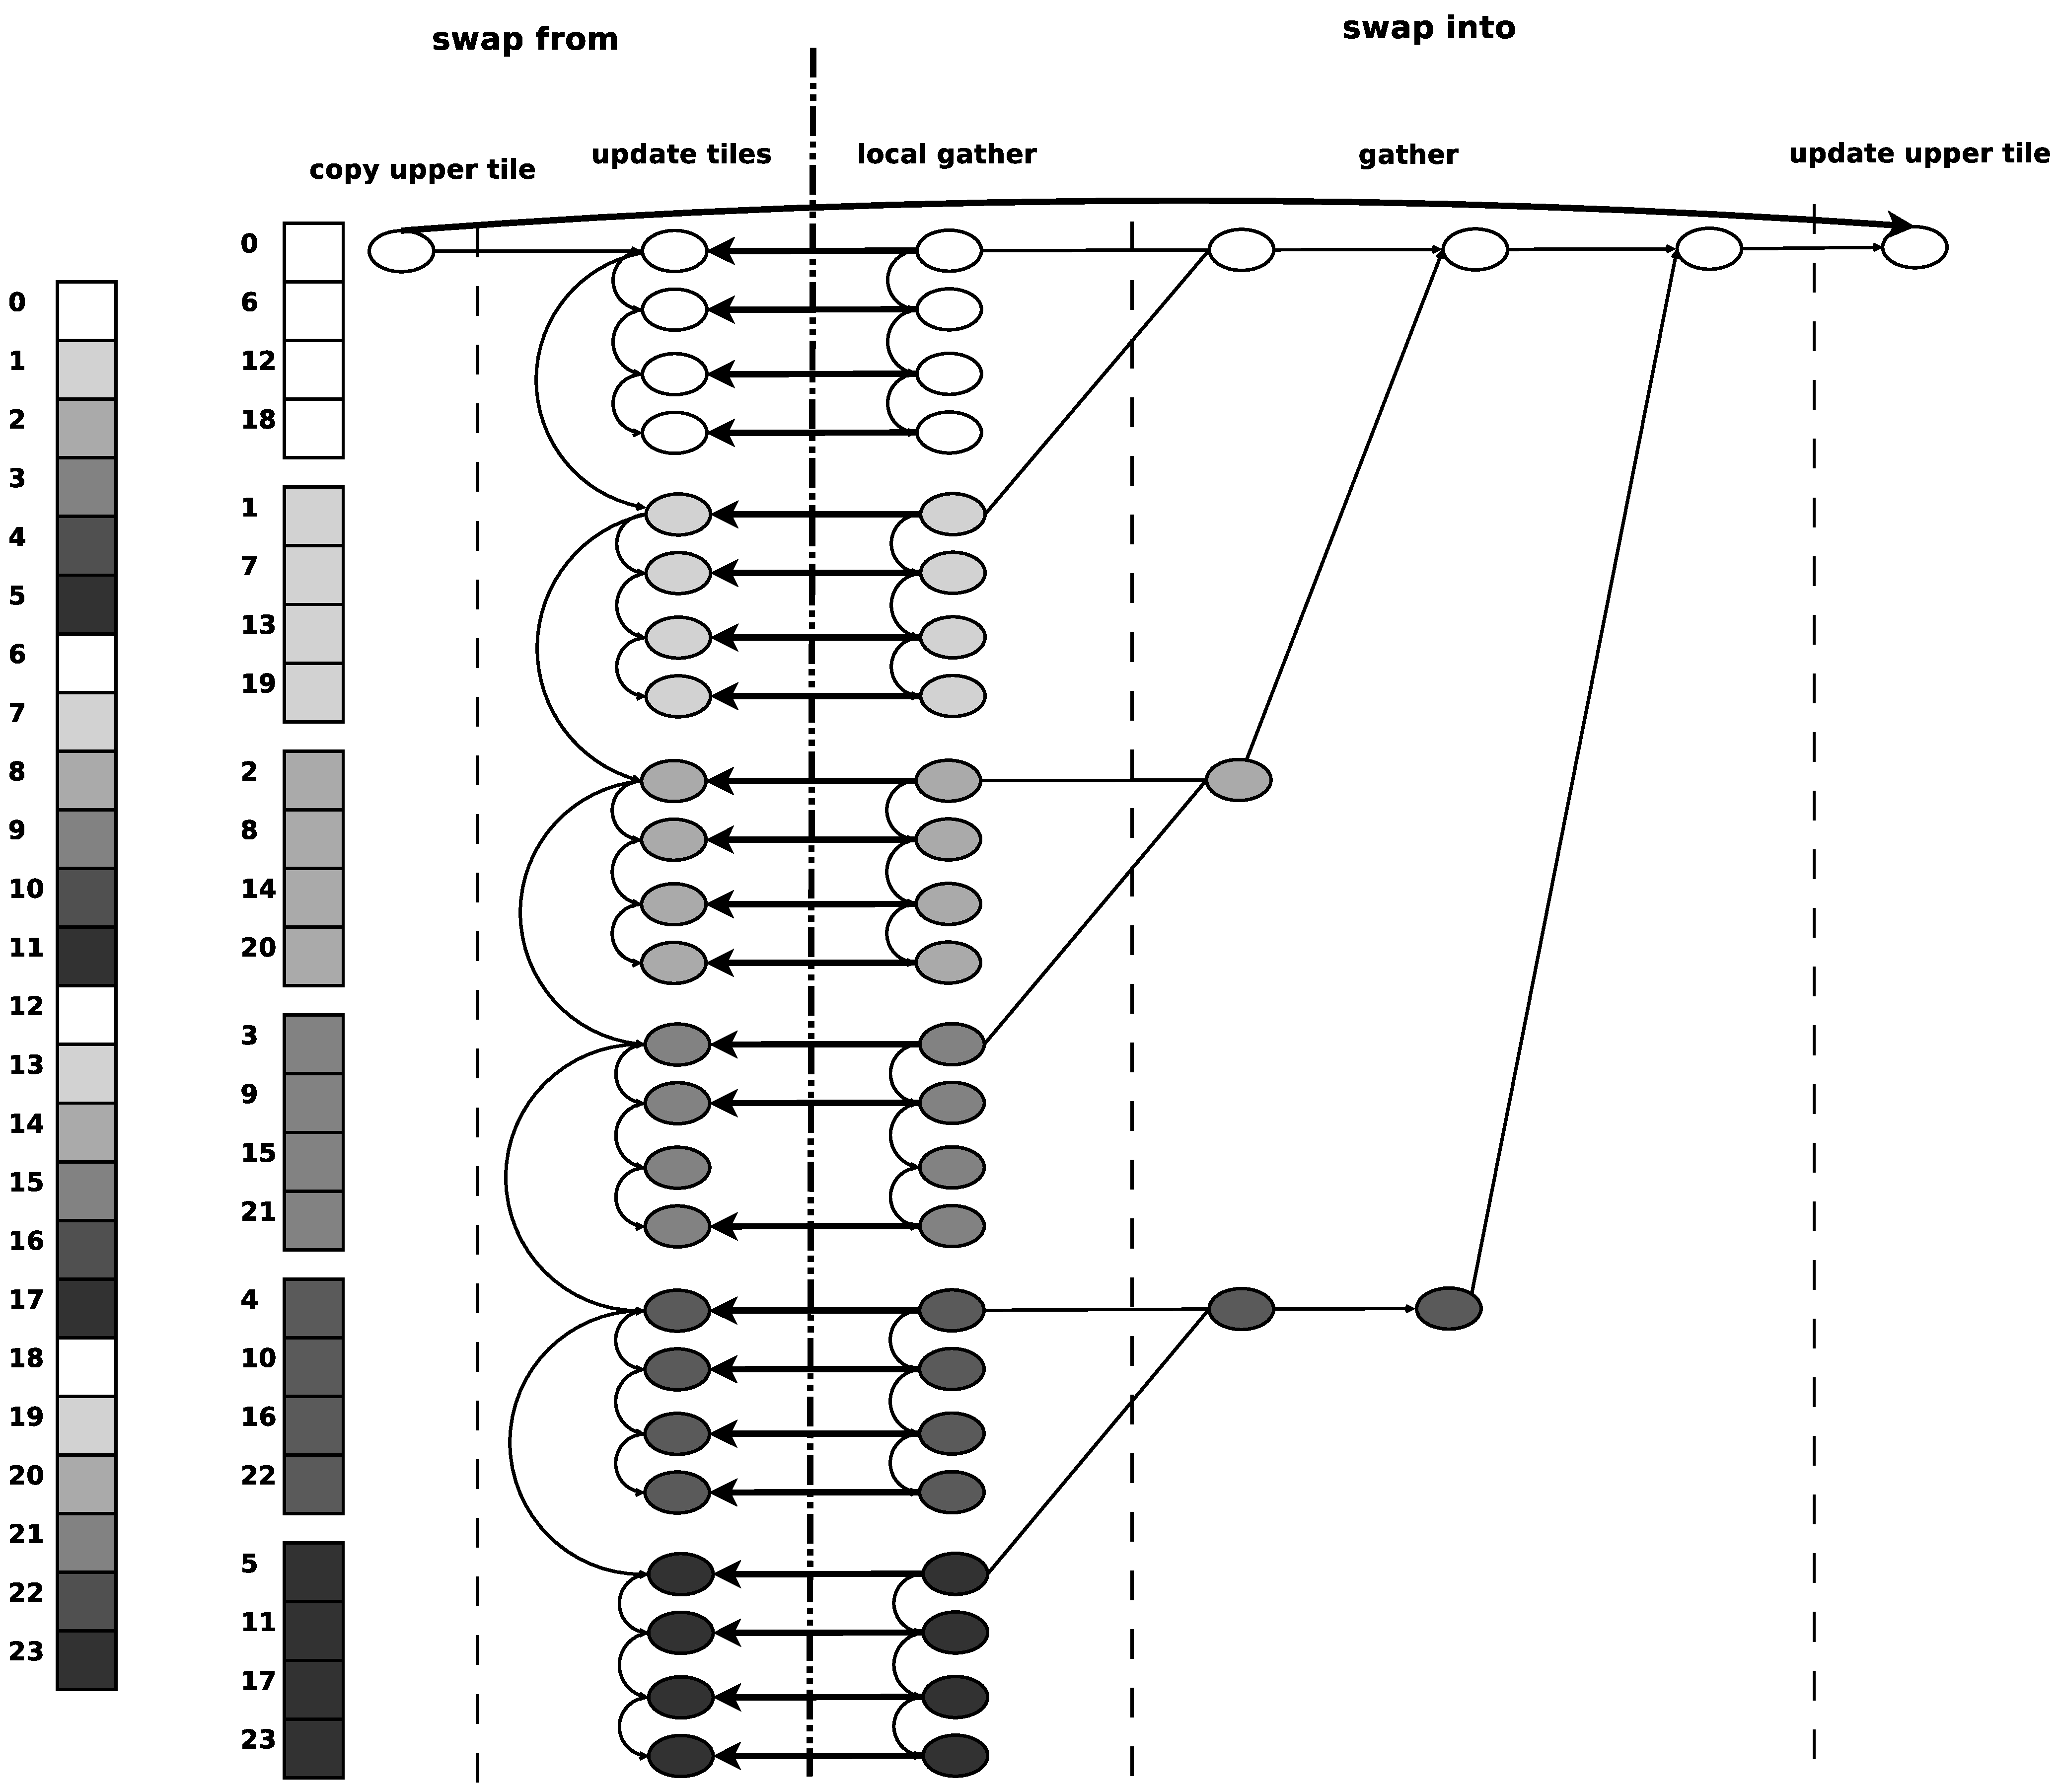
\includegraphics[width=0.65\textwidth]{update_tf_bw}
\end{center}
\end{frame}
